% !TEX root = ../../report.tex
\clearpage
\section{Experimental Plan}
\label{sec:experimental-plan}

%We can sometimes evaluate how well the recommender achieves its overall goals.
%For example, we can check an e-commerce website revenue with and without the
%recommender system and thereby estimate the value of the system to the website.

This section will cover our experimental plan, starting off by looking at the
goals for our experiments. And how we want to get there. The remaining parts of
the section will describe the datasets used for evaluation, our evaluation methodology.
We have the following main goals for our experiment:

\begin{itemize}
	\item Determine the effect of utilizing multiple event types
	\item Determine whether our proposed implicit rating methods improve the recommendation quality over
	binary preference data.
	\item Evaluate the different implicit rating features and attempt to quantify their importance.
	\item Quantify the value of adding a cold-start solution method to the system.
	\item Propose a \emph{best} best combination of methods, given our current limitations for the SoBazar recommender system.
\end{itemize}

As baselines for our project we wish to first test a set of binary methods on the sobazar data
looking only at \emph{purchases}. We do the same for a binary dataset including the events
\emph{purchase}, \emph{wants} and \emph{likes}. We then want to test our \emph{implicit ratings}
considering different factors such as \emph{implicit factor weighting}, \emph{global popularity},
\emph{recency} and factors blended together using different schemes and see if they improve the
recommendation quality.

\subsection{Challenges}

%Every researchers wet dream - online system
The main problem with our experiment is the evaluation part. Namely, how can be determine
whether one set of ratings is better than another, and thereby validating our experiments?
The main reasons for implementing a recommender system is the desire to improve user
satisfaction and to increase the economic
success of a platform. Although both goals are interrelated they may be competing in some
scenarios. The user might be more interested in purchasing the products with the best
price-performance ratio, while the \emph{owners}
are more interested in showing the products that lead to the highest revenue for the
business. For this purpose, a commercial recommender could/should consider implementing
a reward attribute for items that show how much the company profits from its sale. However,
this is something that could be factored in during online testing at a later point.
The following figure shows an overview of the rating evaluation pipeline:

\begin{figure}[H]
		\centering
	  	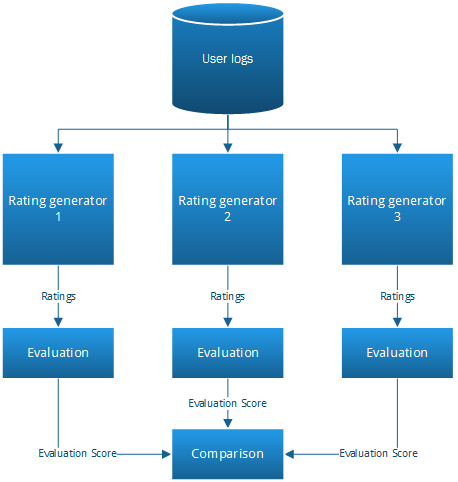
\includegraphics[scale=0.7]{image/ratinggeneval.png}
		\caption[Comparing Ratings]{The Figure shows the process of comparing ratings}
		\label{figure:compareratings}
\end{figure}

In order to further specify our goals we therefore have to take a closer look at the recommender's task,
its interface and the available data. The most typical task for a e-commerce recommender system is to
determine an order of items, often with the purpose of creating a top-k list of items that is shown in a sidebar
or on a dedicated page. The following figure shows the Sobazar newsfeed. Recommendations are likely
to be shown in a similar fashion. The interface currently initially shows four items, but lets the
user scroll sideways over up to 20 items.

\begin{figure}[H]
		\begin{subfigure}[b]{.45\linewidth}
			\centering
	  	
\includegraphics[scale=0.25]{image/SoBazaarfeed2.png}
		\end{subfigure}
		\begin{subfigure}[b]{.45\linewidth}
			\centering
			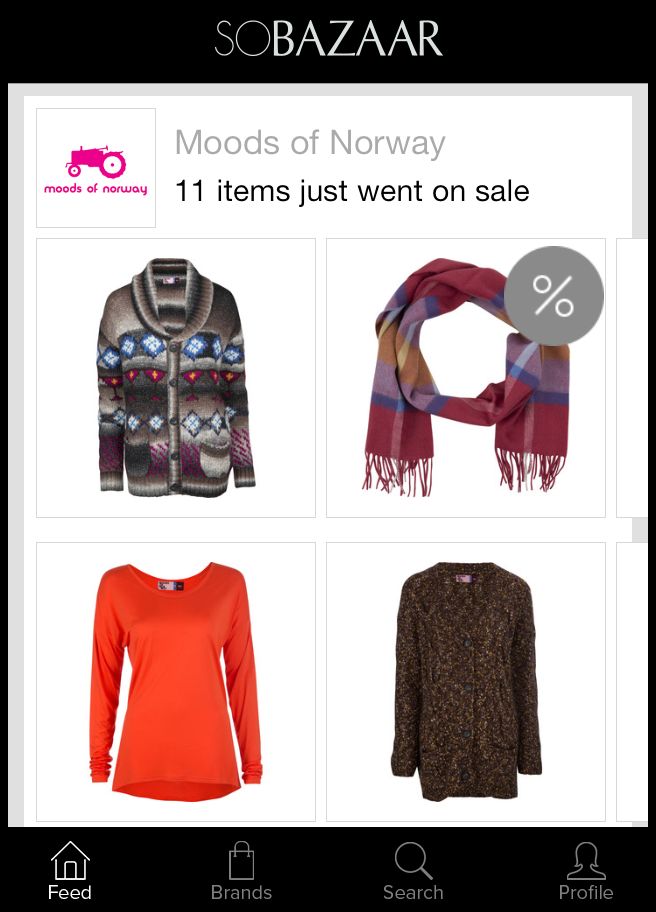
\includegraphics[scale=0.25]{image/SoBazaarsale.png} 
		\end{subfigure}
		\caption[Sobazaar News Feed - Version 0.5.1]{SobBazaar news feed items}
		\label{figure:sobazarfeed}
\end{figure}

Ultimately, the goal of the experiment is to evaluate and measure the properties
of the system, which we have identified as the most important for the systems success,
and select the method that performs the best overall with respect to these properties.

\subsubsection{Dataset}

In addition to evaluate the methods on the Sobazar dataset we want to make sure that our
methods generalizes beyond our experimental dataset, in accordance to the general guidelines
for experimental studies \cite{Shani2011}. The data used for offline evaluation should match
as closely as possible the data we expect the recommender system to face when it is
deployed \cite{Gunawardana2009}. When selecting datasets for evaluation we focused on the
following dataset properties:

\begin{itemize}
	\item Size of dataset: Preferable as close as possible to Sobazar or larger (a few months from now)
	in terms of number of ratings, users and items.
	\item Different different types of implicit factors	such as clicks, likes and purchases.
	\item Domain: Preferably a domain as close to possible as the e-commerce domain where
	factors like recency also would apply.
	\item Timestamps: To evaluate the recentness mapping
	\item Presence of features (Secondary)
\end{itemize}

We were unable to acquire any e-commerce datasets containing user browsing history, purchases etc.
Thus making the main contributions of this article untestable, thus rendering further experiments
on other datasets useless. It is worth nothing that we inquired other researchers having
experimented with similar datasets to no luck.

\paragraph{The Sobazar Dataset}

The Sobazar dataset is small and sparse dataset. When looking only at the purchases
we have a total of 1,592 binary ratings given by 466 users to 1188 items. When including
clicks, wants and purchases we end up with 27,873 ratings given by 1,511 users to 5,855 items.
We also have access to semi-structured product information collected/crawled from
the online retailers for \emph{a majority} items.

Having such a small and sparse dataset has several implications. Firstly we have
to avoid \emph{wishful thinking} as we have very thin data, meaning that we cannot
rely on getting reliable results. Secondly, our evaluation methodology must be
\emph{tailored} for small sparse datasets. E.g. when using cross-validation the number
of folds depends on the size of the dataset. For large datasets, even 3-fold Cross
validation will be quite accurate, while for very sparse datasets, one may have to
use leave-one-out in order to train on as many examples as possible. The advantages
of using a large number of folds is that the bias of the true error rate estimators
will be small, meaning that the estimator will be very accurate, with the disadvantages being that
the variance of the true error rate estimator will be large in addition to increased
computation time. Another alternative well suited for sparse datasets is the \emph{all but one} or the
\emph{leave one out} method, in which we remove one rating from the test users
and try to predict the hidden rating.

Another important concern is whether or not to take the timestamps into consideration,
which directly speaks against the use of cross-validation, as we wish to use the past
interactions to predict future actions. When using the \emph{leave one out} method one
could e.g. always remove the users freshest rating and try to predict it and repeat the
process any number of times. This is particularly relevant as some of our implicit mapping functions
factors in recency.

\subparagraph{Overview of the Dataset}

Table \ref{table:datasets} shows an overview of the sobazar dataset.

%TODO - What else is interesting to know? Rating scale, average number of ratings per user, number of cold start users...
%TODO - % of users with less than 5 ratings for both datasets

\begin{table}[H]
    \centering
    \begin{tabular}{l l l l l l }
    \toprule
	Dataset						& 	Ratings		& 	Users		& 	Items 		& 	Sparsity			& Rating Scale 				    \\ \midrule
	Sobazar	(Purchases Only) 	&	1,592		&	466			&	1188		&	99.71243			& Binary						\\
	Sobazar (All events)		& 	27,873  	& 	1,511		&	5855		& 	99.69657			& Binary/Implicit Ratings		\\ 
	%Movielens 1M				& 	1,000,029   &	6040 		&	3706		&	95.53164			& Explicit (1-5)				\\ 
	\bottomrule
    \end{tabular}
    \caption [Overview of the datasets used for evaluation]{Overview of the datasets used for evaluation}
    \label{table:datasets}
\end{table}

As you can see the recommender can cover a much larger portion of the user group and items when including multiple event types.

\subsection{Comparing Ratings}

The success on our experiment mainly relies on whether we can successfully compare a set of ratings.
Evaluating and comparing a set of ratings is not something you often encounter in the literature. And the
bottom line is that evaluating and comparing a set of ratings is hard. However, we have a few theories on
how it can be done:

\begin{enumerate}
\item Can we put the ratings into a traditional recommender system evaluation pipeline and use the
	  results from that to compare the ratings. In that case, what evaluation metrics are suitable?
\item User studies. Ask users to evaluate how well the produced ratings fit their actual preferences \cite{parra2011walk}.
\item Online experiments measuring e.g. the increased revenue generated or the click-through-rate.
\end{enumerate}

Where we \emph{chose} to go for the first alternative, despite its obvious weaknesses. User studies
are expensive and we simply do not have the time or resources to interview hundreds of actual users.
We do also not have the option of performing any online experiments. Either way it would be best to
get some kind of validation on our results before deploying the system to minimize the risk of giving
low-quality recommendations to the users.

We could say that we believe that better ratings gives us better recommendation results, and use this
as a basis for our evaluation. However, this means that the results we get from testing them
on different algorithms should be comparable. There are two main problems with this. The first is that
we rely on a recommender algorithm can make use of our implicit ratings. We also need to be careful
when selecting evaluation metrics. Many evaluation metrics consider supplied ratings as the \emph{ground truth}
and bases its evaluation score on these numbers. This automatically disqualifies any evaluation metrics
that consider the rating values such as e.g. MAE. After some thought and consideration
we identified the following properties as the best indicators of improved recommendation quality.

\begin{itemize}
\item Does it improve the recall?
\item Does it improve the recommenders ability to rank the items?
\end{itemize}

A further discussion on evaluation metrics will follow in the next Section \ref{sec:eval-metrics}.

\subsubsection{Purchase Only Vs. Multiple Implicit Factors}

\marginpar{I cannot see how we possibly can compare these two...}

We want to evaluate whether a recommender system utilizing multiple implicit factors outperform
a recommender system utilizing purchase data only.
How, then, do we determine one as better than the other? We can see the following challanges:
Firstly, we have two different datasets, as one contains 1045 users and 4667 items more than the
other. How much should the additional coverage factor in? How do we treat the items and users
occurring only in one dataset when evaluating? How do we \emph{treat} the events types only
occurring in one dataset? Only \emph{sensible} thing to do is to compare the purchased items
in some way, the question is how? Currently we can not see how we possibly could compare the
two using traditional offline evaluation methods. Meaning that our comparison of the two will
be made on somewhat of a \emph{subjective} basis.
	
\subsubsection{Comparing Binary and Non-Binary Models}

\marginpar{The question then, is how critical this flaw is to our experiment}
We want to quantify the improvements if any from using implicit ratings over binary ratings.
The main challenges of comparing the binary ratings with the non-binary ones are the fact
that the models for making recommendations differ. Optimally you would like to fix every
\emph{variable} when doing this comparison, however, it is not possible in this case.
To \emph{solve} this problem we decided that the best solution was to select \emph{state-of-the-art}
methods from both classes and compare their results. Worst case scenario we find out that the
methods for non-binary implicit feedback are not as \emph{good} as the binary models and thus
should not be used.

\subsubsection{Comparing Implicit Rating Methods}

%What we want to do
We want to figure out how to evaluate and compare the different implicit rating
methods.  The most obvious solution here would be to analyze the amount of
purchases, wants and clicks in the recommendation lists individually. This is
mainly a evaluation metric problem. Which will be discussed at length in the
next Section.

%Challanges/Problems of actually doing it
%How can we determine if one set of recommendations is better than another?
%	- Evaluation metric problem
%	- One obvious solution would be to analyze the amount of purchases, wants and clicks
%	  in the recommendation lists individually.
%	  	- How much at the list do we take into consideration?
%	  		- 20 is a pretty obvious choice based on the UI of the application
%	  	- How do we weight the different events
%	  	- How do we determine the positional importance of the recommendations?
%	  		- Always recommending purchases in the top positions is better than
%	  		  recommending clicks, but how much better exactly?
%How do we plan to solve them
	%Assumptions & Weaknesses

\subsection{Combining Implicit Ratings With Existing Cold-Start Solutions}

%Only use cold-start splits for this sections tables.

After the best method have been chosen we wish to further improve our results
by adding a cold-start solution to our system. In the second stage of our
experiment we wish to see if we can apply a cold-start solution to increase the
systems cold-start performance.  Here we also wish to factor in factors such as
recency to see whether or not connecting new users with the most popular items
for the $k$ last weeks, instead of the entire period further can improve the
cold-start performance of the system. Similarly for our criticBot where we
can select the most active users for the $n$ last weeks.

\subsubsection{Simulating the Cold-Start Problem}

To simulate the cold-start problem and evaluate how well our the different
methods tackle the different cold-start situations we use the following
evaluation methodology. As mentioned in Section \ref{sec:cold-start-eval} there
is no common framework for assessing the cold-start performance of recommender
systems.  Our goal is to come up with \emph{comprehensive} framework to assess
the cold-start performance of our recommender systems. The following inputs
changes the dataset over time:

\begin{itemize}
	\item 	Existing users watch new items in the catalogue
	\item	New users join the system and view their first item
	\item	New items are added to the catalogue
\end{itemize}

The first input source has the effect of increasing the dataset density, the
average user profile length, and the average number of views per item. The
second input factor has the effect of decreasing both the dataset density and
the average user profile length, as the new users that join the system have
interacted with only a few items. Similarly, the third input factor has the
effect of decreasing both the dataset density and the average number of views
per item.

To simulate the cold-start user problem we propose splitting the users into two
disjoint sets, similarly as in \cite{Stern2009, Lam2008}, using 90\% of the
users for training and setting aside the remaining 10\% for evaluation. We then
train the model with e.g. 5, 15, 25 and 35 of the test users ratings and give
predictions for all models. Alternatively one could train the model using e.g.
25\% and 75\% of each test users ratings. Similarly, to simulate the cold-start
item problem we again split the items into two disjoint sets, using 90\% of the
items for training and the remaining 10\% for evaluation.  We then train the
model with e.g. 20, 40, 60 and 80 ratings and predict the remaining values. The
selection criteria for test items and users can differ from dataset to dataset.
E.g. in \cite{Rashid2002, Rashid2008} the authors selected a subset of the
users with more than 200 ratings, but you can not expect 10\% all the users for
all datasets to have provided 200 ratings, so this number might be lowered if
necessary. The implications of removing the top 10\% of the raters from the
Sobazar dataset is fairly large as they stand for a large portion of the few
ratings we have.

To evaluate the cold-start system performance we use the same method as
described in ~\cite{Agarwal2009} where the authors propose using a 75:25
training/test split, where we at random draw e.g. 35\%, 50\% and then finally
use all (75\%) of the ratings in the training set and predict the remaining
25\%.

%How is this implemented on the sobazar data?

For the Sobazar dataset we select 10\% of the users as test users, for a user
to be selected as a test user, the user must have provided at least 20 ratings.
The test user are drawn at random from the eligible candidates. We then train
the model using 10\%, 40\% and 75\% of their ratings and try to predict their
remaining ratings.  The reason for choosing percentages over hard limits is due
to the fact that the ratings are distributed unevenly among the users. As we
have a very low number of ratings and a large item collection we had to use
only 5\% of the items as test items, where each test item have been rated by
atleast 15 users.  We train the model using 10\%, 40\% and 75\% of their
ratings and try to predict their remaining ratings. As we have access time
timestamps, we split the users and items based on timestamp.  E.g. for the 10\%
user split we train the model with their initial ratings and try to predict
their following ratings. To evaluate the cold-start system performance we split
the dataset in a test and training set using 20\% of the ratings for testing
and then train the model using 40\%, 60\% and 80\% of the ratings for training.
It is important to note that this process should be repeated multiple times, as
the chance of getting an \emph{unfortunate} split is highly probable due to the
dataset size. For the cold-start system task we also split the dataset based on
timestamps, meaning that the test set consists of the most recent ratings.

\begin{center}
    \begin{tikzpicture}
		[node distance = 1cm, auto,font=\footnotesize,
		% STYLES
		every node/.style={node distance=1.5cm},
		% The comment style is used to describe the characteristics of each process
		comment/.style={rectangle, 
										inner sep= 5pt,
										text width=3cm,
										node distance=0.25cm,
										font=\scriptsize\sffamily},
		% small comment lol
		comment-small/.style={rectangle,
													inner sep= 5pt,
													text width=1cm,
													node distance=0.25cm,
													font=\scriptsize\sffamily},
		% The nonProcess style
		nonProcess/.style={rectangle,
											 draw,
											 inner sep=5pt,
											 text width=3cm,
											 text badly centered,
											 minimum height=1.2cm,
											 font=\footnotesize\sffamily},
		% The process style is used to draw the processs' name
		process/.style={rectangle,
										draw,
										fill=black!10,
										inner sep=5pt,
										text width=3cm,
										text badly centered,
										minimum height=1.2cm,
										font=\bfseries\footnotesize\sffamily},
		% ratingsGenerator style
		ratingsGenerators/.style={rectangle,
															draw,
															fill=blue!50,
															inner sep=5pt,
															text width=3cm,
															text badly centered,
															minimum height=1.2cm,
															font=\bfseries\footnotesize\sffamily},
		% racommendation algorithms
		recAlgs/.style={rectangle, draw, fill=red!40, inner sep=5pt, text width=3cm, text badly centered, minimum height=1.2cm, font=\bfseries\footnotesize\sffamily}]

		% Draw processs
		\node [ratingsGenerators] (rg1) {popularity};
		\node [ratingsGenerators, right=0.25 of rg1] (rg2) {price};
		\node [comment-small, right=0.01 of rg2] (dotdotdot) {..............};
		\node [ratingsGenerators, right=0.01 of dotdotdot] (rg3) {recentness};
		\node [process, below of=rg2] (gt) {"Ground Truth"};
		\node [recAlgs, below of=gt] (ra2) {ALS};
		\node [recAlgs, left=0.25 of ra2] (ra1) {KNN};
		\node [comment-small, right=0.01 of ra2] (dotdotdot2) {..............};
		\node [recAlgs, right=0.01 of dotdotdot2] (ra3) {wALS};
		\node [process, below of=ra2] (eval) {Evaluation Score};
		\node [comment, right=0.25 of rg3] (comment-rg3) {
			Implicit ratings
		};
		\node [comment, right=0.25 of ra3] (comment-ra3) {
			Recommendations algorithm
		};
		% Draw the links between processs
		\path[->,thick]
			(rg1) edge (gt)
			(rg2) edge (gt)
			(dotdotdot) edge (gt)
			(rg3) edge (gt)
			(gt) edge (ra1)
			(gt) edge (ra2)
			(gt) edge (dotdotdot2)
			(gt) edge (ra3)
			(ra1) edge (eval)
			(ra2) edge (eval)
			(dotdotdot2) edge (eval)
			(ra3) edge (eval);
		\draw[>=latex,->] (gt) -- +(-6,0) |- (eval);
    \end{tikzpicture}
    \captionof{figure}[Implicit Rating Evaluation]{Overview of how the generated ratings from the implicit feedback can be evaluated.}
  	\label{figure:implicitRatingEvaluation}
  \end{center}

The blue boxes in figure~\ref{figure:implicitRatingEvaluation} are functions
used to produce the implicit ratings based on the implicit feedback. Based on
this, the system gets an estimated \emph{ground truth}, which can be used to
evaluate the different recommendation algorithms show in the red boxes. Based
on the evaluation score something can be said about the implicit feedback
conversion to implicit ratings and the recommendation algorithms used.
